%
% firmware.tex
%
% Copyright (C) 2021 by Universidade Federal de Santa Catarina.
%
% OBDH 2.0 Documentation
%
% This work is licensed under the Creative Commons Attribution-ShareAlike 4.0
% International License. To view a copy of this license,
% visit http://creativecommons.org/licenses/by-sa/4.0/.
%

%
% \brief Firmware chapter.
%
% \author Gabriel Mariano Marcelino <gabriel.mm8@gmail.com>
%
% \institution Universidade Federal de Santa Catarina (UFSC)
%
% \version 0.10.0
%
% \date 2019/10/30
%

\chapter{Firmware} \label{ch:firmware}

\section{Product tree}

The product tree of the firmware part of the OBDH 2.0 module is available in \autoref{fig:product-tree-fw}.

\begin{figure}[!ht]
    \begin{center}
        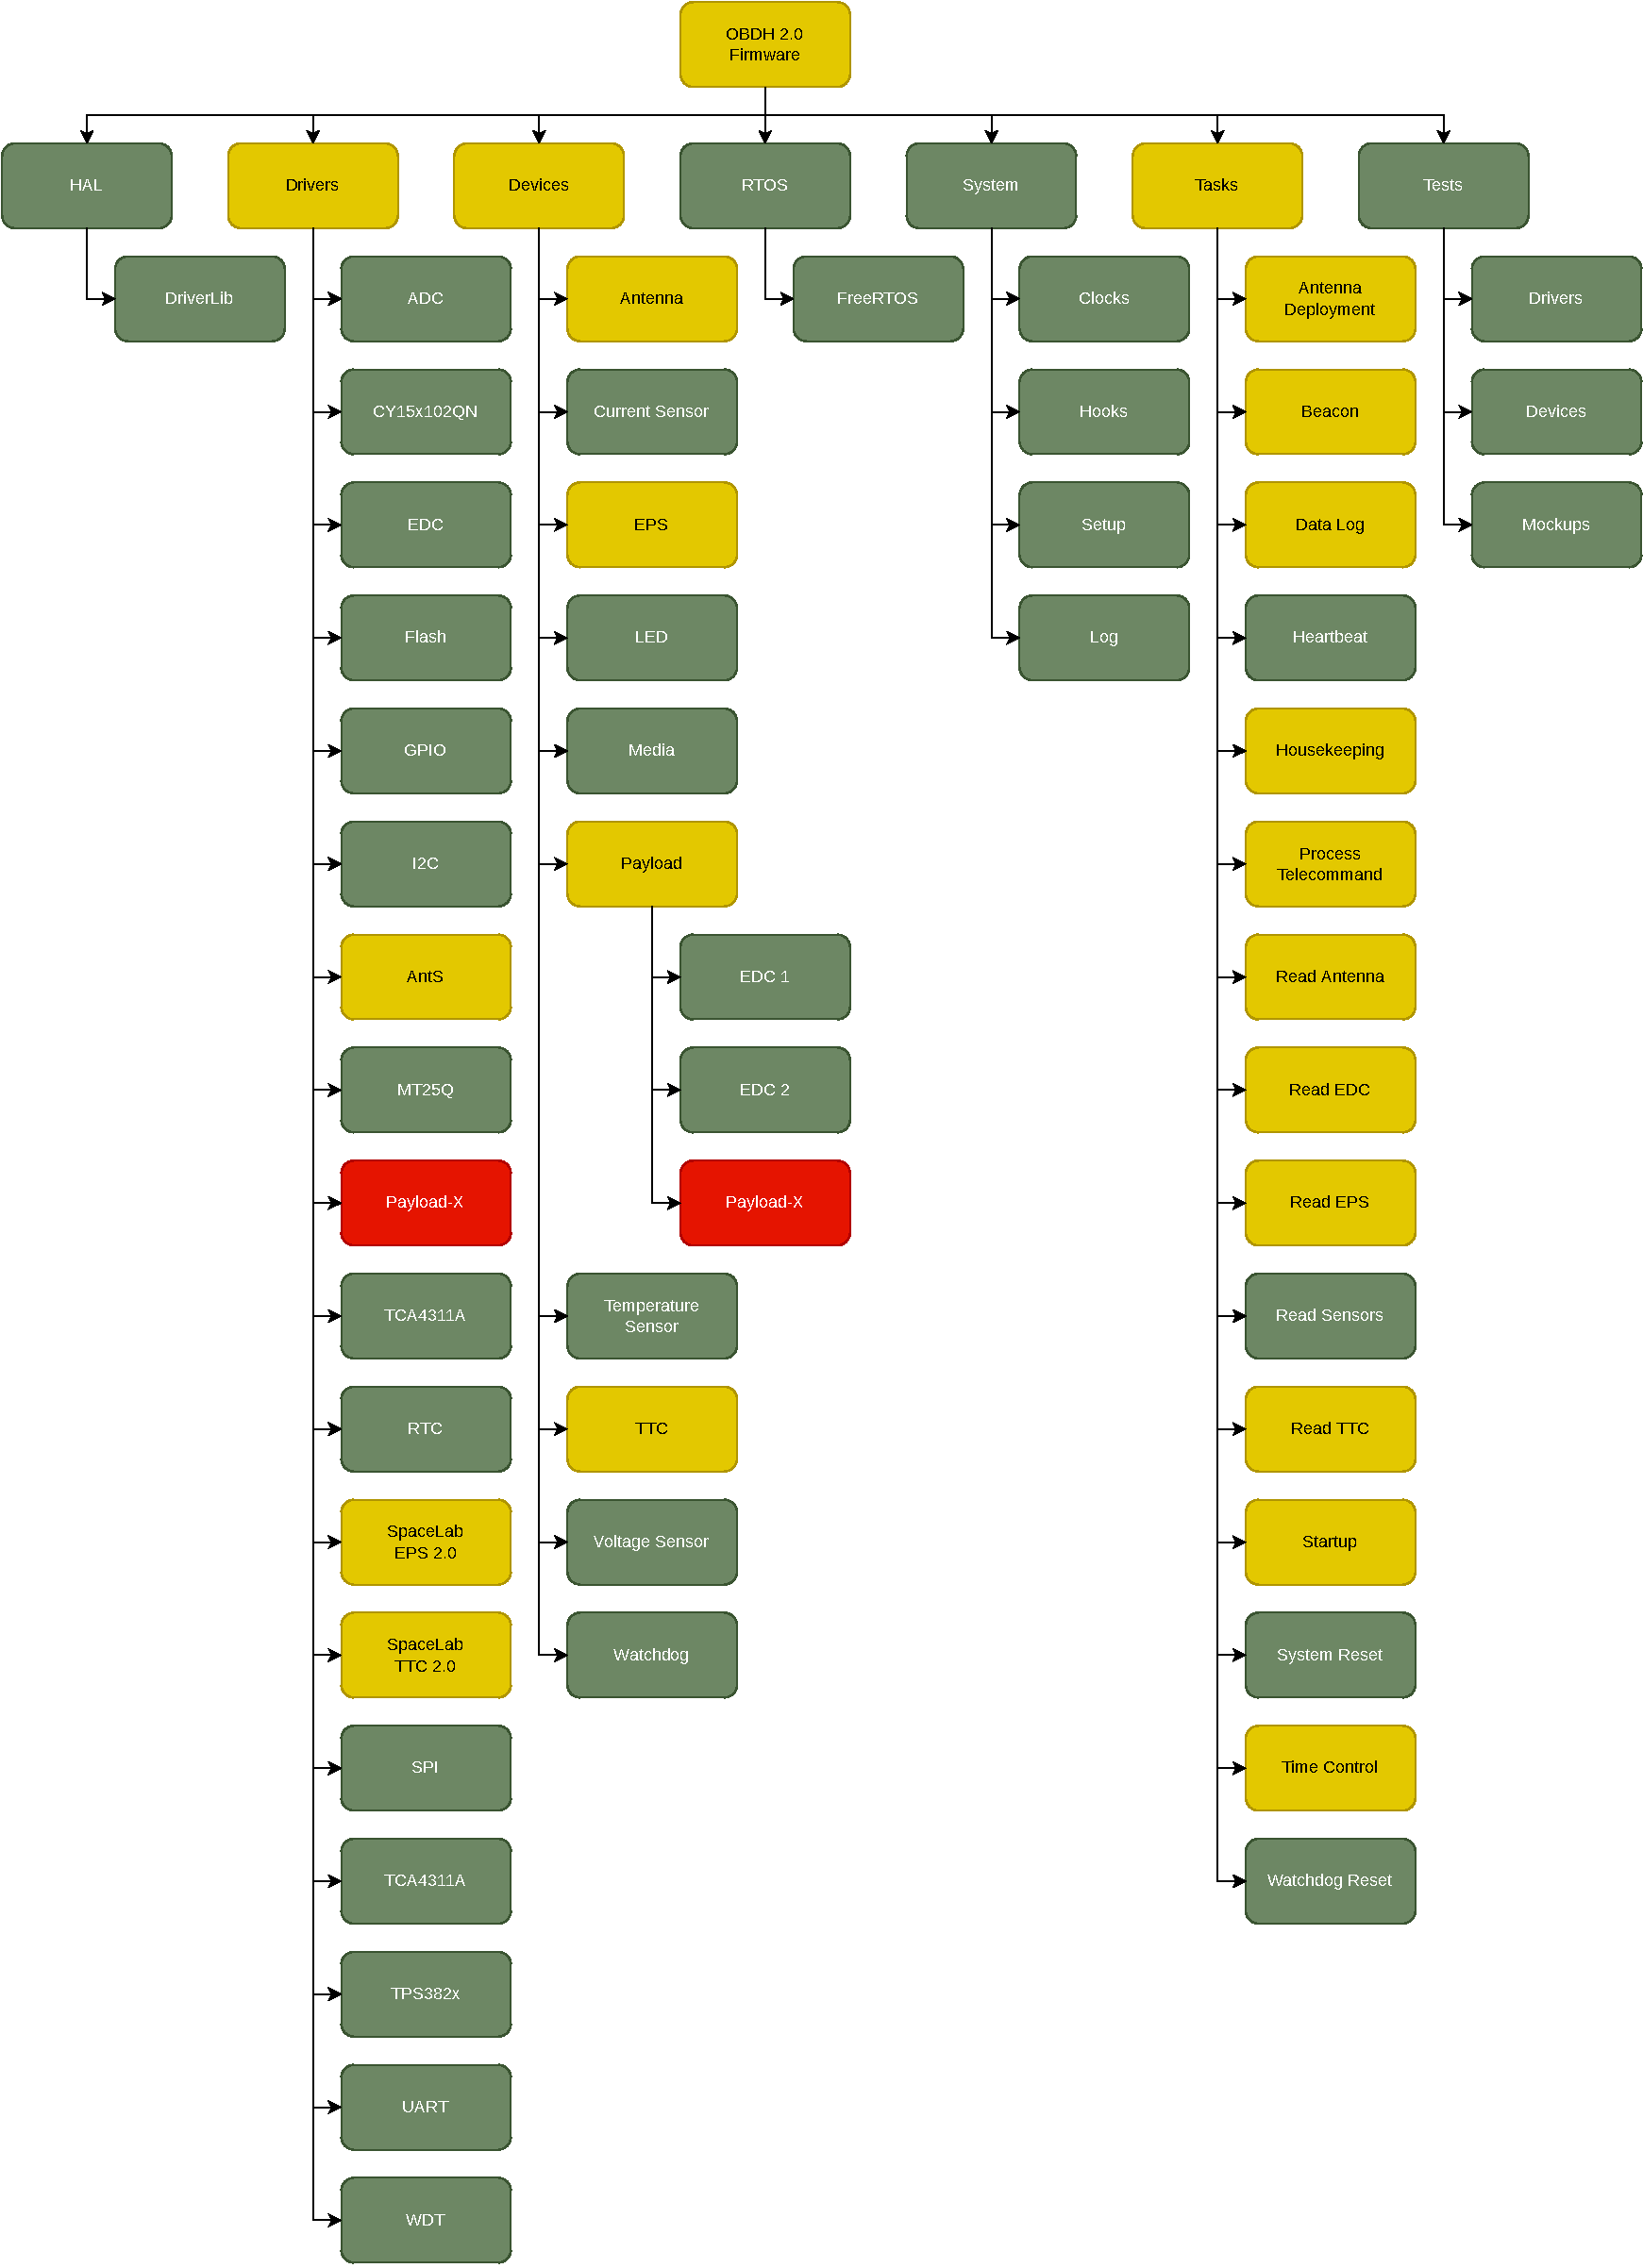
\includegraphics[width=\textwidth]{figures/product-tree-fw.pdf}
        \caption{Product tree of the firmware of the OBDH 2.0 module.}
        \label{fig:product-tree-fw}
    \end{center}
\end{figure}

\section{Dependencies}

The firmware depends on external libraries to access the embedded hardware or to communicate with other modules. A list of these libraries and the used version is available in \autoref{tab:fw-dependencies}.

\begin{table}[!ht]
    \centering
    \begin{tabular}{L{5cm}R{4cm}}
        \toprule[1.5pt]
        \textbf{Library}        & \textbf{Version} \\
        \midrule
            MSP430 DriverLib    & v2.91.11.01 \\
            FreeRTOS            & v10.2.1 \\
        \bottomrule[1.5pt]
    \end{tabular}
    \caption{External libraries and dependencies of the firmware.}
    \label{tab:fw-dependencies}
\end{table}

\section{Tasks}

A list of the firmware tasks can be seen in the \autoref{tab:firmware-tasks}.

\begin{table}[!ht]
    \centering
    \begin{tabular}{lccccc}
        \toprule[1.5pt]
        \textbf{Name} & \textbf{Priority} & \textbf{Initial delay [ms]} & \textbf{Period [ms]} & \textbf{Stack [bytes]} \\
        \midrule
        Antenna deployment     & Highest & 0      & Aperiodic & 150  \\
        Antenna reading        & Medium  & 2000   & 60000     & 150  \\
        Beacon                 & High    & 10000  & 60000     & 1000 \\
        Data log               & Medium  & 2000   & 600000    & 225  \\
        EDC reading            & Medium  & 2000   & 60000     & 300  \\
        EPS reading            & Medium  & 2000   & 60000     & 384  \\
        Heartbeat              & Lowest  & 2000   & 500       & 160  \\
        Housekeeping           & Medium  & 2000   & 10000     & 160  \\
        Read sensors           & Medium  & 2000   & 60000     & 140  \\
        Startup (boot)         & Highest & 0      & Aperiodic & 350  \\
        System reset           & Medium  & 0      & 36000000  & 128  \\
        Telecommand processing & High    & 10000  & 5000      & 500  \\
        Time control           & Medium  & 1000   & 1000      & 128  \\
        TTC reading            & Medium  & 2000   & 60000     & 384  \\
        Watchdog reset         & Lowest  & 0      & 100       & 150  \\
        \bottomrule[1.5pt]
    \end{tabular}
    \caption{Firmware tasks.}
    \label{tab:firmware-tasks}
\end{table}

All these tasks are better described below.

\subsection{Antenna deployment}

This task deploys the Antenna module at the start of the mission.

\subsection{Antenna reading}

Reads the Antenna module status.

\subsection{Beacon}

The Beacon task transmits a data package containing the satellite's basic telemetry data every 60 seconds.

\subsection{Data log}

This task saves the housekeeping data of the satellite in flash memory every 10 minutes.

\subsection{EDC reading}

This task reads all the EDC packages and data.

\subsection{EPS reading}

This task reads all the EPS data and status.

\subsection{Heartbeat}

The heartbeat task keeps blinking a LED (``\textit{System LED}'' in \autoref{fig:status-leds}) at a rate of 1 Hz during the execution of the system. Its purpose is to give visual feedback on the execution of the scheduler. This task does not have a specific purpose on the flight version of the module (the flight version of the PCB does not have LEDs).

\subsection{Housekeeping}

This task reads all the important OBDH data and status.

\subsection{Read sensors}

This task reads the internal sensors of the OBDH every 60 seconds.

\subsection{Startup (boot)}

This task is the first executed task when the system starts. All devices, libraries, and data structures are initialized in this task. When the execution is done, the remaining tasks of the system are allowed to execute.

\subsection{System reset}

This task resets the microcontroller by software every 10 hours. This can be useful to clean up possible wrong values in variables, repeat the antenna deployment routine (limited to $n$ times), clean up the RAM, etc.

\subsection{Telecommand processing}

This task processes all the telecomands; it needs to have a really short period for a more responsive operation.

\subsection{Time control}

This task is responsible for the time management of the system. At every second, it increments the system time (epoch). Also, it saves the current system time in the non-volatile memory every minute.

\subsection{TTC reading}

This task reads all the TTC data and status.

\subsection{Watchdog reset}

This task resets the internal and external watchdog timer every 100 ms. The internal watchdog has a maximum count time of 500 ms, and the external watchdog has a maximum of 1600 ms (see \autoref{ch:hardware} for more information about the watchdog timers).

To prevent the system to not reset during an anomaly on some task (like an execution time longer than planned), this task has the lowest possible priority: 0.

\section{Variables and Parameters}

The internal variables and parameters of the OBDH firmware can be seen in \autoref{tab:vars-and-pars}.

\begin{longtable}[c]{cL{0.82\textwidth}l}
    \toprule[1.5pt]
    \textbf{ID} & \textbf{Name/Description} & \textbf{Type}\\
    \midrule
    0   & Time counter in milliseconds                            & uint32 \\
    1   & Temperature of the $\mu$C in Kelvin                     & uint16 \\
    2   & Input current in mA                                     & uint16 \\
    3   & Input voltage in mV                                     & uint16 \\
    \multirow{18}{*}{4} & Last reset cause: & \multirow{18}{*}{uint8} \\
        & - 0x00 = No interrupt pending                           &        \\
        & - 0x02 = Brownout (BOR)                                 &        \\
        & - 0x04 = RST/NMI (BOR)                                  &        \\
        & - 0x06 = PMMSWBOR (BOR)                                 &        \\
        & - 0x08 = Wakeup from LPMx.5 (BOR)                       &        \\
        & - 0x0A = Security violation (BOR)                       &        \\
        & - 0x0C = SVSL (POR)                                     &        \\
        & - 0x0E = SVSH (POR)                                     &        \\
        & - 0x10 = SVML\_OVP (POR)                                &        \\
        & - 0x12 = SVMH\_OVP (POR)                                &        \\
        & - 0x14 = PMMSWPOR (POR)                                 &        \\
        & - 0x16 = WDT time out (PUC)                             &        \\
        & - 0x18 = WDT password violation (PUC)                   &        \\
        & - 0x1A = Flash password violation (PUC)                 &        \\
        & - 0x1C = Reserved                                       &        \\
        & - 0x1E = PERF peripheral/configuration area fetch (PUC) &        \\
        & - 0x20 = PMM password violation (PUC)                   &        \\
        & - 0x22 to 0x3E = Reserved                               &        \\
    5   & Reset counter                                           & uint16 \\
    6   & Last valid telecommand (uplink packet ID)               & uint8  \\
    7   & Temperature of the radio in Kelvin                      & uint16 \\
    8   & RSSI of the last valid telecommand                      & uint16 \\
    9   & Temperature of the antenna in Kelvin                    & uint16 \\
    \multirow{17}{*}{10} & Antenna status bits: & \multirow{17}{*}{uint16}  \\
        & - Bit 15: The antenna 1 is deployed (0) or not (1)      &        \\
        & - Bit 14: Cause of the latest activation stop for antenna 1 &    \\
        & - Bit 13: The antenna 1 deployment is active (1) or not (0) &    \\
        & - Bit 11: The antenna 2 is deployed (0) or not (1)      &        \\
        & - Bit 10: Cause of the latest activation stop for antenna 2 &    \\
        & - Bit 9: The antenna 2 deployment is active (1) or not (0)  &    \\
        & - Bit 8: The antenna is ignoring the deployment switches (1) or not (0) & \\
        & - Bit 7: The antenna 3 is deployed (0) or not (1)       &        \\
        & - Bit 6: Cause of the latest activation stop for antenna 3 &     \\
        & - Bit 5: The antenna 3 deployment is active (1) or not (0) &     \\
        & - Bit 4: The antenna system independent burn is active (1) or not (0) & \\
        & - Bit 3: The antenna 4 is deployed (0) or not (1)       &        \\
        & - Bit 2: Cause of the latest activation stop for antenna 4 &     \\
        & - Bit 1: The antenna 4 deployment is active (1) or not (0) &     \\
        & - Bit 0: The antenna system is armed (1) or not (0)     &        \\
    11  & Hardware version                                        & uint8 \\
    12  & Firmware version (ex.: ``v1.2.3'' = 0x00010203)         & uint32 \\
    13  & Mode (``Normal'' = 0, ``Hibernation'' = 1)              & uint8 \\
    14  & Timestamp of the last mode change                       & uint32 \\
    15  & Mode duration in sec. (valid only in hibernation mode)  & uint32 \\
    16  & Initial hibernation executed                            & boolean \\
    17  & Initial hibernation time counter (minutes)              & uint8 \\
    18  & Antenna deployment executed                             & boolean \\
    19  & Antenna deployment counter                              & uint8 \\
    \bottomrule[1.5pt]
    \caption{Variables and parameters of the OBDH 2.0.}
    \label{tab:vars-and-pars}
\end{longtable}

\section{Telemetry}


\subsection{Beacon}

The beacon packet is transmitted every 1 minute and contains basic telemetry data of the satellite. The content of this packet can be seen in \autoref{tab:telemetry-beacon}.

\begin{itemize}
    \item Period: 60 seconds
    \item Band: UHF
    \item Condition to operate: Always on
\end{itemize}

\begin{table}[!ht]
    \centering
    \begin{tabular}{llc}
        \toprule[1.5pt]
        \textbf{Parameter} & \textbf{Content}       & \textbf{Length [bytes]} \\
        \midrule
        Packet ID          & 10h                    & 1 \\
        Satellite callsign & ``0PY0EGU''            & 7 \\
        $\mu$C temperature & Raw $\mu$C temperature & 2 \\
        $\mu$C voltage     & Raw $\mu$C voltage     & 2 \\
        $\mu$C current     & Raw $\mu$C current     & 2 \\
        Last reset cause   & Last reset cause ID    & 1 \\
        System time        & System time in ticks   & 4 \\
        Radio temperature  & Raw radio temperature  & 4 \\
        Last TC RSSI       & Raw RSSI value         & 2 \\
        Last received TC   & Last received TC ID    & 1 \\
        Battery 1 voltage  & Raw battery 1 voltage  & 2 \\
        Battery 2 voltage  & Raw battery 2 voltage  & 2 \\
        Battery current    & Raw battery current    & 2 \\
        Battery charge     & Raw battery charge     & 2 \\
        % ...                & ...                    & ... \\
        \midrule
        Total              & -                      & 34 \\
        \bottomrule[1.5pt]
    \end{tabular}
    \caption{Beacon packet.}
    \label{tab:telemetry-beacon}
\end{table}

\subsection{EDC Information}

Telemetry packages from EDC can be seen in \autoref{tab:telemetry-edc}.

\begin{table}[!ht]
    \centering
    \begin{tabular}{llc}
        \toprule[1.5pt]
        \textbf{Parameter} & \textbf{Content}                                 & \textbf{Len. [bytes]} \\
        \midrule
        Packet ID          & 11h                                              & 1 \\
        Satellite callsign & ``0PY0EGU''                                      & 7 \\
        \midrule
        \multicolumn{3}{c}{\textbf{PTT Decoder}} \\
        \midrule
        Time tag           & PTT signal receiving time                        & 4 \\
        Error code         & Error code                                       & 1 \\
        Carrier frequency  & Carrier frequency                                & 2 \\
        Carrier Abs        & Carrier amplitude at ADC interface output        & 2 \\
        Message length     & User message length in bytes                     & 1 \\
        User message       & ARGOS-2 PTT-A2 user message                      & 35 \\
        \midrule
        \multicolumn{3}{c}{\textbf{HK Info}} \\
        \midrule
        Current time       & Current time since J2000 epoch                   & 4 \\
        Elapsed time       & Elapsed time since last reset                    & 4 \\
        Current supply     & System current supply in mA                      & 2 \\
        Voltage supply     & System voltage supply in mV                      & 2 \\
        Temperature        & EDC board temperature                            & 1 \\
        PLL sync bit       & RF front end LO...                               & 1 \\
        ADC RMS            & RMS level at front-end output                    & 2 \\
        Num of RX PTT      & Generated PTT packages since last initialization & 1 \\
        Max                &                                                  & 1 \\
        Memory error count &                                                  & 1 \\
        \midrule
        \multicolumn{3}{c}{\textbf{System State}} \\
        \midrule
        Current time       &                                                  & 4 \\
        PTT available      & Number of PTT Package available for reading      & 1 \\
        PTT is paused      & PTT decoder task status                          & 1 \\
        Sampler state      & ADC sampler state                                & 1 \\
        \midrule
        Total              & -                                                & 79 \\
        \bottomrule[1.5pt]
    \end{tabular}
    \caption{EDC information packet.}
    \label{tab:telemetry-edc}
\end{table}

\subsection{EDC Samples}

The EDC samples are \textcolor{red}{TBD} bytes long and are transmitted in Y packets with 219 bytes each.

\begin{table}[!ht]
    \centering
    \begin{tabular}{llc}
        \toprule[1.5pt]
        \textbf{Parameter} & \textbf{Content}               & \textbf{Length [bytes]} \\
        \midrule
        Packet ID          & 12h                            & 1 \\
        Satellite callsign & ``0PY0EGU''                    & 7 \\
        Time tag           & Elapsed time since J2000 epoch & 4 \\
        Packet counter     & ADC sample packet number       & 1 \\
        I sample[n]        & First ADC I-sample             & 2 \\
        Q sample[n]        & First ADC Q-sample             & 2 \\
        ...                & ...                            & ... \\
        I sample[n+102]    & First ADC I-sample             & 2 \\
        Q sample[n+102]    & First ADC Q-sample             & 2 \\
        \midrule
        Total              & -                              & 219 \\
        \bottomrule[1.5pt]
    \end{tabular}
    \caption{EDC samples packet.}
    \label{tab:telemetry-edc-samples}
\end{table}

\section{Telecommands}

The system telecommands can be seen in \autoref{tab:system-telecommands}.

\begin{table}[!ht]
    \centering
    \begin{tabular}{lll}
        \toprule[1.5pt]
        \textbf{Name}          & \textbf{Parameters}           & \textbf{Access} \\
        \midrule
        Enter hibernation      & Hibernation period in seconds & Private         \\
        Leave hibernation      & None                          & Private         \\
        Activate beacon        & None                          & Private         \\
        Deactivate beacon      & None                          & Private         \\
        Activate downlink      & None                          & Private         \\
        Deactivate downlink    & None                          & Private         \\
        Activate EDC           & None                          & Private         \\
        Deactivate EDC         & None                          & Private         \\
        Get EDC info           & None                          & Private         \\
        Activate Radiation instrument     & Experiment period in seconds  & Private         \\
        Deactivate Radiation instrument   & None                          & Private         \\
        Set system time        & Time value (epoch)            & Private         \\
        Ping                   & None                          & Public          \\
        Message broadcast      & ASCII message                 & Public          \\
        Request data           & Data flags                    & Public          \\
        \bottomrule[1.5pt]
    \end{tabular}
    \caption{System telecomamnds.}
    \label{tab:system-telecommands}
\end{table}

\subsection{Enter hibernation}

This telecommand activates the hibernation mode in a satellite. During the hibernation mode, no transmissions are made by the satellite, it keeps just listening for new incoming packets (reception). The satellite will stay in hibernation mode for a custom period (1 to 65536 minutes), or until a ``Leave Hibernation'' mode is received. This is a private telecommand, a key is required to send it. Beyond the packet ID and the source callsign (or address), the number o minutes (2 bytes long) is also transmitted.

\begin{table}[!ht]
    \centering
    \begin{tabular}{lll}
        \toprule[1.5pt]
        \textbf{Parameter}      & \textbf{Content}                         & \textbf{Length [bytes]} \\
        \midrule
        Packet ID               & 20h                                      & 1 \\
        Ground station callsign & Any callsign (ASCII, filled with ``0''s) & 7 \\
        Hibernation period      & Period in minutes (1 to 65535)           & 2 \\
        Key                     & Telecommand key (ASCII)                  & 10 \\
        \midrule
        Total                   & -                                        & 20 \\
        \bottomrule[1.5pt]
    \end{tabular}
    \caption{Enter hibernation telecommand.}
    \label{tab:enter-hibernation-tc}
\end{table}

\subsection{Leave hibernation}

This telecommand complements the ``enter hibernation'' telecommand by deactivating the hibernation mode in the satellite. When a satellite receives this telecommand it enables the transmission again immediately. This is also a private telecommand; a specific key is required to send it. There is no additional content to this telecommand packet, just the packet ID and the source callsign (or address).

\begin{table}[!ht]
    \centering
    \begin{tabular}{lll}
        \toprule[1.5pt]
        \textbf{Parameter}      & \textbf{Content}                         & \textbf{Length [bytes]} \\
        \midrule
        Packet ID               & 21h                                      & 1 \\
        Ground station callsign & Any callsign (ASCII, filled with ``0''s) & 7 \\
        Key                     & Telecommand key (ASCII)                  & 10 \\
        \midrule
        Total                   & -                                        & 18 \\
        \bottomrule[1.5pt]
    \end{tabular}
    \caption{Leave hibernation telecommand.}
    \label{tab:leave-hibernation-tc}
\end{table}

\subsection{Activate beacon}

This telecommand activates the beacon transmissions.

\subsection{Deactivate beacon}

This telecommand deactivates the beacon transmissions.

\subsection{Activate EDC}

This telecommand activates the EDC payload.

\subsection{Deactivate EDC}

This telecommand deactivates the EDC payload.

\subsection{Get EDC info}

This telecommand request information from the EDC payload. When received, the OBDH transmits the housekeeping and state frames of the EDC module (28 bytes). This telecommand does not require a key.

\subsection{Activate Module}

The ``Activate Module'' telecommand is a command to activate an internal module of the satellite. Each module has a unique ID that is passed as an argument of this telecommand's packet. The \autoref{tab:activate-module-table} shows the current used IDs.
This is also a private telecommand, and a key is required to transmit it.

\begin{table}[!ht]
    \centering
    \begin{tabular}{lll}
        \toprule[1.5pt]
        \textbf{Module}     & \textbf{ID number} \\
        \midrule
        Battery heater      & 1 \\
        Beacon              & 2 \\
        Periodic telemetry  & 3 \\
        \bottomrule[1.5pt]
    \end{tabular}
    \caption{Leave hibernation telecommand.}
    \label{tab:activate-module-table}
\end{table}

\subsection{Deactivate Module}

The ``Deactivate Module'' telecommand complements the telecommand above. It works the same way and with the same parameters, but in this case, it has the purpose of deactivating a given module of the satellite.

\subsection{Activate Radiation Instrument}

This telecommand activates the Radiation Instrument.

\subsection{Deactivate Radiation Instrument}

This telecommand deactivates the Radiation Instrument.

\subsection{Activate Payload}

This telecommand is similar to the telecommand ``Activate Module'', but in this case is used for the activate payloads of the satellite. Each satellite will have a list of IDs of the set of payloads.

This is also a private telecommand, and a key is required to transmit it.

\subsection{Deactivate Payload}

Same as the ``Deactivate Module'' telecommand, but for payloads.

\subsection{Erase Memory}

The telecommand ``erase memory'' erases all the content presented in the non-volatile memories of the onboard computer of a satellite. This is a private command, and a key is required to send it. No additional content is required in a erase memory telecommand packet, just the packet ID and the source callsign (or address).

\subsection{Force Reset}

This telecommand performs a general reset of the satellite. When received, the satellite reset all subsystems. This is a private telecommand, and a key is required to send this command to a satellite. There is no additional content in this packet, just the packet ID and the source callsign (or address).

\subsection{Get Payload Data}

This telecommand allows a ground station to download data from a specific satellite payload. The required fields are the payload ID, and, optionally, arguments to be passed to the payload. The IDs and arguments vary according to the satellite. This is a private telecommand, and a key is required to send it.

\subsection{Set Parameter}

This telecommand allows the configuration of specific parameters of a given satellite subsystem. The required fields are the ID of the subsystem to set (1 byte), the ID of the parameter to set (1 byte), and the new value of the parameter (4 bytes long). The possible IDs (subsystem and parameter) vary according to the satellite. This is a private telecommand, and a key is required to send it.

\subsection{Get Parameter}

The telecommand ``Get Parameter'' complements the ``Set Parameter'' telecommand. It has the purpose of reading specific parameters of a given subsystem. The required fields are the subsystem's ID (1 byte) and the parameter ID (1 byte). The possible IDs (subsystem and parameter) vary according to the satellite. This is a private telecommand, and a key is required to send it.

\subsection{Set system time}

This telecommand sets the internal system time. This is useful for synchronizing the satellite time with a ground station installed on Earth.

\subsection{Ping}

The ping request telecommand is a simple command to test the communication with the satellite. When the satellite receives a ping packet, it will respond with another ping packet (with another packet ID, as defined in the downlink packets list). There are no additional parameters in the ping packet, just the packet ID and the source callsign (or address). It is also a public telecommand; anyone can send a ping request telecommand to a satellite.

\begin{table}[!ht]
    \centering
    \begin{tabular}{lll}
        \toprule[1.5pt]
        \textbf{Parameter}      & \textbf{Content}                         & \textbf{Length [bytes]} \\
        \midrule
        Packet ID               & 22h                                      & 1 \\
        Ground station callsign & Any callsign (ASCII, filled with ``0''s) & 7 \\
        \midrule
        Total                   & -                                        & 8 \\
        \bottomrule[1.5pt]
    \end{tabular}
    \caption{Ping telecommand.}
    \label{tab:ping-tc}
\end{table}

\begin{table}[!ht]
    \centering
    \begin{tabular}{lll}
        \toprule[1.5pt]
        \textbf{Parameter}      & \textbf{Content}                               & \textbf{Length [bytes]} \\
        \midrule
        Packet ID               & 12h                                            & 1 \\
        Satellite callsign      & ``PY0EGU''                                     & 7 \\
        Destination callsign    & Requester callsign (ASCII, filled with ``0''s) & 7 \\
        \midrule
        Total                   & -                                              & 15 \\
        \bottomrule[1.5pt]
    \end{tabular}
    \caption{Ping telecommand answer.}
    \label{tab:ping-tc-ans}
\end{table}

\subsection{Message broadcast}

The ``broadcast message'' is another public telecommand; no authentication or key is required to send this telecommand to a satellite. This command has the purpose of making a satellite transmit a custom message back to Earth. This can be useful for communication tasks, like a station sending data to another. There are two parameters in this telecommand: the destination callsign (or address), and the content of the message, which can be any sequence of ASCII characters or any byte value. There is a limit of 38 characters in the message field. The \autoref{tab:msg-broadcast-tc} shows the Telecommand parameters.

\begin{table}[!ht]
    \centering
    \begin{tabular}{lll}
        \toprule[1.5pt]
        \textbf{Parameter}      & \textbf{Content}                         & \textbf{Length [bytes]} \\
        \midrule
        Packet ID               & 23h                                      & 1 \\
        Ground station callsign & Any callsign (ASCII, filled with ``0''s) & 7 \\
        Message                 & Message to broadcast (ASCII)             & up to  \\
        \midrule
        Total                   & -                                        & 8 \\
        \bottomrule[1.5pt]
    \end{tabular}
    \caption{Message broadcast telecommand.}
    \label{tab:msg-broadcast-tc}
\end{table}

\subsection{Request data}

The data request telecommand is a command to download data from the satellite. This command allows a ground station to get specific parameters from a given period (stored in the satellite's non-volatile memory of the onboard computer). The list of possible parameters varies according to the satellite. The required fields of this telecommand are the parameter ID (1 byte), the start period in milliseconds (epoch, 4 bytes), and the end period in milliseconds (epoch, 4 bytes). This is a private telecommand, and a key is required to send it.

\section{Operating System}

The FreeRTOS 10 \cite{freertos} is being used as an operating system. FreeRTOS is a market-leading real-time operating system (RTOS) for microcontrollers and small microprocessors. Distributed freely under the MIT open-source license, FreeRTOS includes a kernel and a growing set of IoT libraries suitable for use across all industry sectors. FreeRTOS is built with an emphasis on reliability and ease of use.

The main configuration parameters of the operating system in this project are available in \autoref{tab:freertos-config}.

\begin{table}[!ht]
    \centering
    \begin{tabular}{lrr}
        \toprule[1.5pt]
        \textbf{Parameter}       & \textbf{Value} & \textbf{Unit} \\
        \midrule
        Version                  & v10.2.0        & - \\
        Tick rate (Hz)           & 1000           & Hz \\
        CPU clock (HZ)           & 32             & MHz \\
        Max. priorities          & 5              & - \\
        Heap size                & 40960          & bytes \\
        Max. length of task name & 20             & - \\
        \bottomrule[1.5pt]
    \end{tabular}
    \caption{FreeRTOS main configuration parameters.}
    \label{tab:freertos-config}
\end{table}

More details of the used configuration parameters can be seen in the file \textit{\href{https://github.com/spacelab-ufsc/obdh2/blob/master/firmware/config/FreeRTOSConfig.h}{firmware/config/FreeRTOSConfig.h}} from \cite{obdh2-repo}.

\section{Hardware Abstraction Layer (HAL)}

As the Hardware Abstraction Layer (HAL\nomenclature{\textbf{HAL}}{\textit{Hardware Abstraction Layer.}}), the DriverLib \cite{driverlib} from Texas Instruments is begin used. It is the official API to access the registers of the MSP430 microcontrollers.

The DriverLib is meant to provide a ``software'' layer to the programmer to facilitate a higher programming level than direct register accesses. By using the high-level software APIs provided by DriverLib, users can create powerful and intuitive code that is highly portable between devices within the MSP430 platform and different families in the MSP430/MSP432 platforms.

%\section{Memory Management}

%\textcolor{red}{TBD}

%\section{
